
{Single cell RNAseq global proportion of resistant vs sensitive clones presented high \textit{in trans}-regulated gene expression variations than \textit{in cis}-regulated genes.}

\subsubsection{Gene co-expression network analysis apprise biological processes relationship}


- Contrasting Frequencies and Effects of cis- and trans-Regulatory Mutations Affecting Gene Expression (read this paper)


%-------------------------------------------------------------

*ASPH \cite{li2018expression, hou2018recent, kanwal2020aspartate, lin2019asph}
CDKN2A \cite{shahidsales2018genetic}-also tumor suppressor??
*RAB10 \cite{wang2017rab10}RAB10 overexpression promotes tumor growth and indicates poor prognosis of hepatocellular carcinoma
Recently, Rab10 has been demonstrated to be aberrantly expressed in some types of cancers and show biological significance in cancer progression \cite{he2002identification, jiang2016mir}
*UBE3C \cite{xiong2019mir, pan2015ubiquitin, zhang2020ube3c}
*YY1 \cite{wan2012yin, chinnappan2009transcription, meliala2020biological} 
YY1 is generally overexpressed in breast cancer cells and tissues.
YY1 was uniformly highly over-expressed in a wide range of human cancer cell lines and in human colon cancer tissue samples.
PFDN-   Prefoldin 1 promotes EMT and lung cancer progression by suppressing cyclin A expression
Overexpression of Canonical Prefoldin Associates with the Risk of Mortality and Metastasis in Non-Small Cell Lung Cancer. 
%-------------------------------------------------------------

- we determine whether under neutral conditions when there is no drug pressure what proportion of the transcriptomes might be copy number driven just due to the natural evolution of the copy number clones. This allows us to understand the stability of the gene expression in our timeseries models in the absence of drugs. 
 Next, we explored that if a drug being introduced into the system, how much of the drug induced change in expression is dependent on the copy number and which are independent.
%-------------------------------------------------------------
SA1035- from regression and gene network analysis:

*UQCRB-
Mitochondrial UQCRB as a new molecular prognostic biomarker of human colorectal cancer \cite{kim2017mitochondrial}

*MDK-Midkine (MDK) growth factor: a key player in cancer progression and a promising therapeutic target

SA535-cisplatin:

*BCAP31- BCAP31 drives TNBC development by modulating ligand-independent EGFR trafficking and spontaneous EGFR phosphorylation
-BCAP31, a cancer/testis antigen-like protein, can act as a probe for non-small-cell lung cancer metastasis
- BCAP31, a cancer/testis antigen-like protein, can act as a probe for non-small-cell lung cancer metastasis

*TPT1-LncRNA TPT1‐AS1 promotes tumorigenesis and metastasis in epithelial ovarian cancer by inducing TPT1 expression

*OLA1-Obg-like ATPase 1 (OLA1) overexpression predicts poor prognosis and promotes tumor progression by regulating P21/CDK2 in hepatocellular carcinoma

- Assessment of the role of translationally controlled tumor protein 1 (TPT1/TCTP) in breast cancer susceptibility and ATM signaling

*METTL5-Roles of METTL3 in cancer: mechanisms and therapeutic targeting
- Ribosome 18S m(6)A Methyltransferase METTL5 Promotes Translation Initiation and Breast Cancer Cell Growth.

*PABPC1-PABPC1 exerts carcinogenesis in gastric carcinoma by targeting miR-34c
-Expression and prognostic roles of PABPC1 in esophageal cancer: correlation with tumor progression and postoperative survival

*MARCKS-Overexpression of MARCKS indicates a poor prognosis of oral squamous cell carcinoma
-Stromal Expression of MARCKS Protein in Ovarian
Carcinomas Has Unfavorable Prognostic Value
-reported increased levels of phospho-MARCKS in clinical specimens of patients with lung cancer
-A novel predictor of cancer malignancy: up-regulation of myristoylated alanine-rich C kinase substrate phosphorylation in lung cancer

*RAC3 -Rac3 induces a molecular pathway triggering breast cancer \cite{gest2013rac3}.
 The Rho GTPases form 8 subfamilies; one subfamily comprises Rac1, Rac2, Rac3 and RhoG; the second subfamily contains Cdc42, TC10 (also known as RhoQ)
 It also was founded that RAC3 overexpression is required to maintain telomerase activity \cite{larrosa2015rac3, chan2005roles}.




%-------------------------------------------------------------









Activation of the interferon alpha signaling pathway has been shown to contribute to apoptosis and cellular senescence but is also attributed to increased migration and drug resistance depending on the interferon-stimulated genes transcribed. The mechanisms promoting the increase in interferon alpha expression and the role interferon alpha plays in IBC remain speculative. Deciphering the role of interferon alpha signaling and microenvironment crosstalk in inflammatory breast cancer
Olivia K. Provance & Joan Lewis-Wambi 
Breast Cancer Research volume 21, Article number: 59 (2019) 
\cite{provance2019deciphering}
\cite{mojic2018dark}-interferon gamma

E2F function couples proliferation and DNA repair by coordinating the induction of genes required for DNA synthesis, such as thymidine kinase (TK1) and dihydrofolatereductase (DHFR), and DNA repair, such as BRCA1, BRCA2, and RAD51 (51).
E2F binds to and regulates the promoters of multiple genes involved in cell cycle progression (e.g., cyclin E and cyclin A) \cite{wiedemeyer2014reversing, knudsen2010targeting}.

- Checkpoint kinase inhibitor AZD7762 enhance cisplatin-induced apoptosis in osteosarcoma cells
- Cell cycle checkpoint in cancer: a therapeutically targetable double-edged sword-G2M pathway upregulated related text.






%The important features of a timeseries patient-derived xenografts  that differentiate it from cross-sectional data-collection procedures \cite{kaplan1995time}:
 
 %\textbf{(a)} Repeated measurements of a given behavior are taken across time at equally spaced intervals.Taking multiple measurements is essential for understanding any given behavior is forced to evolve over time, and doing so at equal intervals give an open opportunity to clearly investigate the dynamics of that behavior manifesting at distinct time scales.
 %\textbf{(b)} The temporal ordering of measurements is preserved. Doing so is the only way to fully examine the dynamics governing a particular process. If we expect that a specific event will influence the dynamics of clones in a particular way, utilizing summary statistics will completely ignore the temporal ordering of the data and likely occlude one’s view of important behavioral dynamics.

%the relative contribution of these processes when  studied  in  tandem  is  poorly  understood  and  requires  integrated  genome-transcriptome investigation.   Moreover,  how  changes  in  genomic  architecture  brought  about  by  copy  number alterations drive etiologic processes remains understudied. Perturbations to induce fitness changes include genetic editing with cancer gene mutations, and pharmacologic drug selection to profile kinetics of therapeutic response.

While transcription phenotype clusters tracked with genotypic clones in the untreated series (\reffig{fig:exp}), analysis of scRNAseq from the parallel treated samples indicated that phenotypes were also impacted by cisplatin (Pearson correlation of \texttt{DLP+} clones and \texttt{clonealign} scRNAseq clones = 0.99, \refsupfig{sfig:rx_10x}A). Global transcription effects generating increased phenotypic volume\cite{Azizi2018-eb} (\reffig{fig:rxexp}A) and transcriptional velocity\cite{La_Manno2018-az} (\reffig{fig:rxexp}B and \refsupfig{sfig:rx_10x}B) were observed as a function of time on treatment.  As nearly all tumour cells were clone R from \textit{X5 UTT} onwards in the treatment series, we attributed transcriptional changes to phenotypic plasticity (\reffig{fig:rxexp}C,D and \refsupfig{sfig:rx_10x}C,D). Globally,  27 genes exhibited monotonic linear and coordinated activity as a function of time on treatment (\reffig{fig:rxexp}C).
Modified pathways included previously confirmed cisplatin-resistance metabolic processes such as oxidative phosphorylation \cite{lee2017myc}, TNFA signaling via NFKB \cite{lagunas2008nuclear,ito2015down,ryan2019targeting}, E2F targets \cite{zheng2020upregulation} and hypoxia \cite{lee2012hypoxia,mcevoy2015identifying,deben2018hypoxia,li2019erk} (\refsuptab{stab:pathway}). From these pathways specific gene expression trajectories (\reffig{fig:rxexp}E) exemplified systematic response to sustained treatment, relative to the untreated and holiday regimes. A minor component of the phenotypic volume was reversible (\reffig{fig:rxexp}A) on drug holiday, indicating only modest or partial reversibility of gene expression of clone R (\reffig{fig:rxexp}E, X5-X6, X6-X7, Rx and Rx-H) for some genes (\textit{CEBP}, \textit{NDUF7}, \textit{MYC}).

Together, these data show the impact of cisplatin selective pressure on the starting tumour cell population is reversible while genomic clonal competition with precursor clones is still possible, but becomes fixed once the evolutionary bottleneck narrows and purifies the population. Once fixed, a minor component of the expression landscape remains reversible. Thus, cisplatin resistance occurred in phases - first dominated by clonal selection on mixed populations, followed by transcriptional plasticity on a fixed genotype.



Then we get percentage of incis, intrans: nb\_incis/total [cosmic,cisplatin,fitness] genes * 100,  nb\_trans/total [cosmic,cisplatin,fitness] genes * 100, and voila, we have this proportion genes plots, blah blah







In spite of advanced technologies and treatment, triple negative breast cancer still facing the problems of tumor recurrence and drug resistance.
For any given difference between the types of drug resistance, for example, the expression of a particular gene, it is assumed that differences arise deterministically or probabilistically in the configuration of transcription factors regulating the genes in the tumors. Cancer cells in distinct cell- states often exhibit important differences in functional properties depending on the which genes are turned on and off resulting in sensitive or resistant phenotype.

The most challenging analysis is to differentiate whether the change in gene expression leading to change in cellular state is stochastic\cite{raj2008nature} and random or its deterministic to produce the same output under similar environment.
Cancer cells in distinct cell- states often exhibit important differences in functional properties depending on which genes are turned on and off resulting in sensitive  or resistant phenotype.
Previously it is shown that unique cells within a population can exhibit fluctuations in expression of a group of genes, that could predict distinct phenotypes \cite{shaffer2019memory}.
Un-like genomic clones that could get selected in resistant phenotype \cite{salehi2020single}, we still are not clear whether the cell-states are acquainted for this kind of behaviour or the selected states are pre-existing in the cancer population and under continues pressure shows obvious dynamics or there is a transition from one state to another that ultimately gets selected over time. Because of difficulty to analyse longitudinal patient's samples for single cell gene expression and lack of multiple longitudinal pre-clinical breast cancer models, these questions remains unexplored.

The introduction of RNA velocity in single cells has opened up new ways of studying cellular differentiation. Time derivative of the gene expression state can be directly estimated by distinguishing unspliced and spliced mRNAs in common single-cell RNA sequencing protocols. RNA velocity is a high-dimensional vector that predicts the future state of individual cells on a timescale of hours.......
Here we set to examine three breast cancer patient derived xenografts (PDX) that were serially challenged for around 4-5 cycles with platinum compound until they started showing resistant behaviour. We wanted to understand the magnitude of fluctuations in gene expression from sensitive to resistant phenotype.


\begin{figure}
\centering
 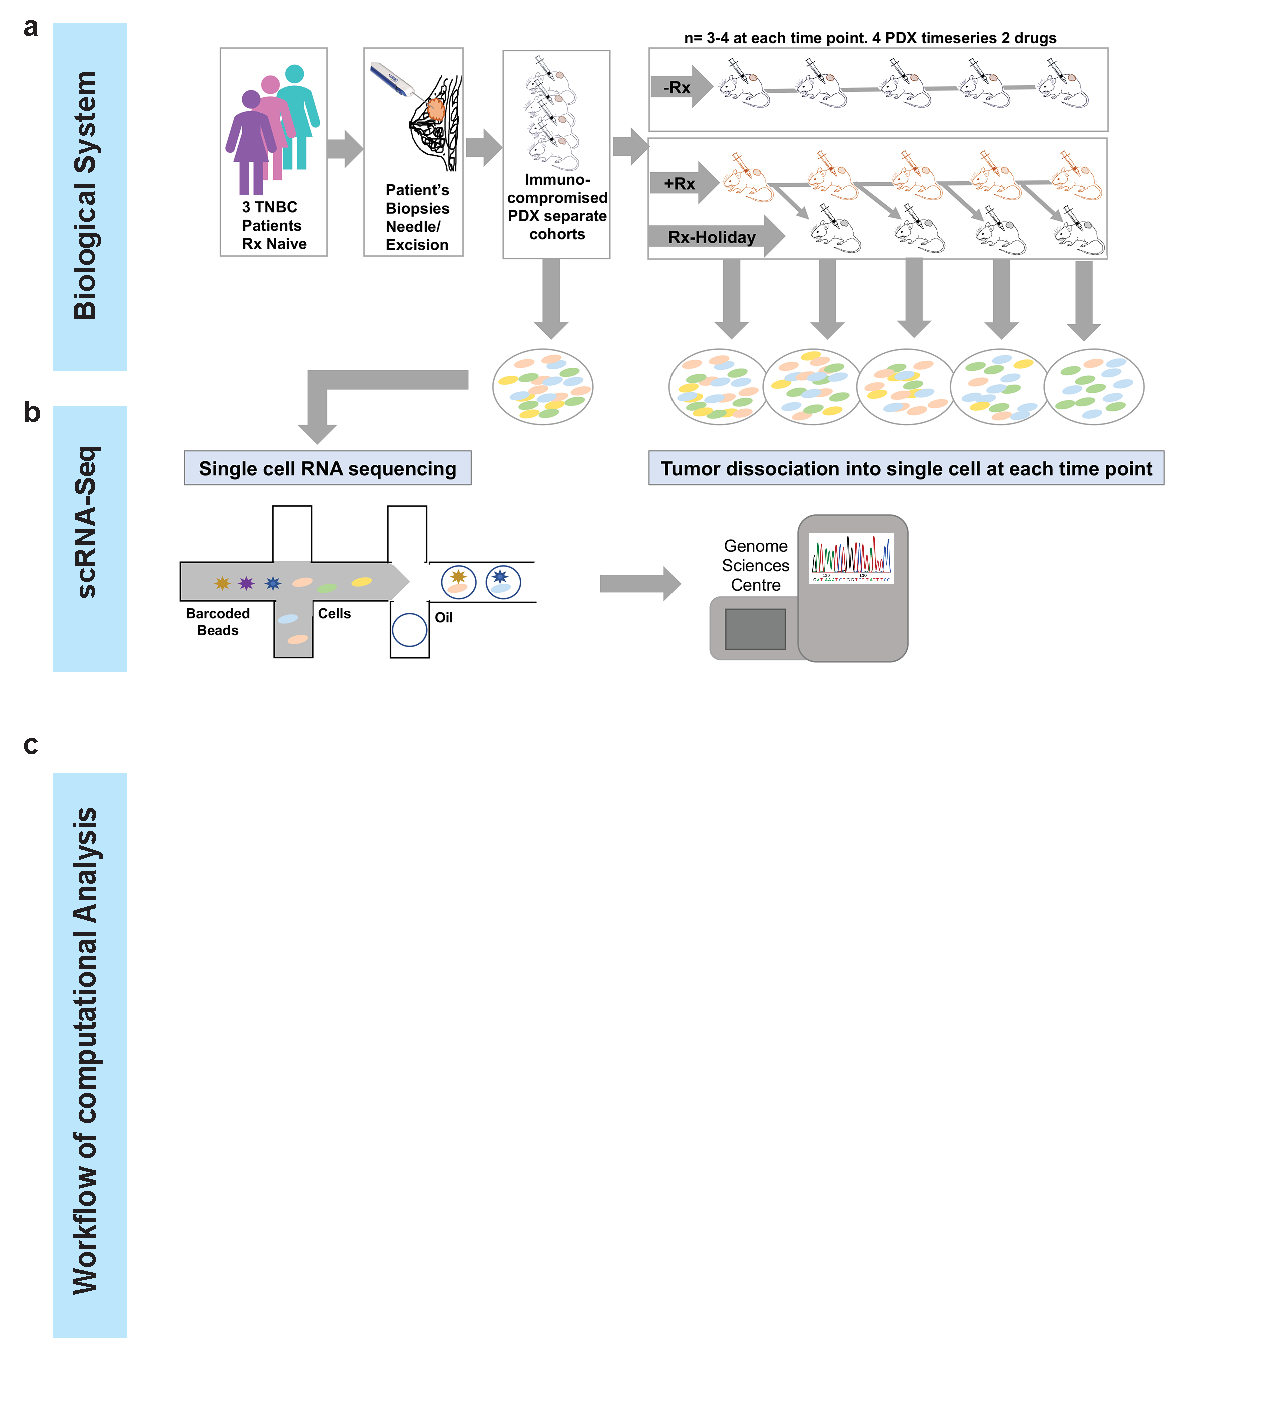
\includegraphics[width=\textwidth]{Figures/fig1schematicsoverview.pdf}
	
\caption[Schematic overview of experimental design and single cell RNA seq data analysis]
	{\small
	 \textbf{Schematic overview of experimental design and single cell RNA seq data analysis} .
	     
	}
	\label{fig:fig1schematicsoverview}
\end{figure}









Dynamics of single cell genomes and transcriptomes in response to chemotherapies

Chapter 1. To discern the stability and reproducibility of drug response properties  
1.1. To understand the range of drug response of breast cancer cell lines with respect to DNA repair deficiency- exploring NHEJ pathway in vitro for CX-5461 mechanism-(co-author paper published in Nature communication)
1.2. Large scale screening of CX-5461 in pooled cancer cell lines to discover genotype-specific vulnerabilities (on going at Broad institute)
1.3. To understand the range of drug response of breast cancer PDX in vitro
1.4. Optimization of PDX tumor processing and freezing techniques for SC whole genome, SC PBAL and SC RNA sequencing. (co-author 3 manuscripts on BioRxiv) 
1.5. Identification of tissue handling on sc-RNA seq- (co-first author manuscript in prep.)
1.6. Dissecting the maximum tolerable drug doses in NRG mice?
1.7. What are the basic patterns of drug sensitivity in PDX in vivo? (on-going)

Chapter 2. Characterizing the fitness of cancer cell in time and space

Understanding the evolutionary process within a tumor (Co-first author- “Fitness” manuscript in preparation)
1.1. Estimating the quantitative fitness of clones from time series sampling of PDX without perturbation
1.2. Do we see the same clones evolving if we physically mix early and late passages at two different dilutions?
1.3. Can we observe any change in clonal dynamics with drug perturbation? (Taxol on SA609)
1.4. What are the growth dynamics of the serially passaged PDX tumors?
1.5. Describing phenotype of all passages of PDX tumors through histological staining and expression at certain time points (SC-RNA-seq) 

Chapter 3. To understand the convergence or divergence of clonal dynamics under chemotherapeutic drugs’ selection (“lineage under drug selection” manuscript outlined)
1.1. Estimating the quantitative fitness of clones from time series sampling of PDX with drug perturbation (SA604, SA609, SA535, SA1035)
1.2.  Do the same clones mediate drug resistance or sensitivity over multiple instances of the same PDX (Using genomic markers of lineage at single cell level)
1.3. Can we compare the lineages to be compared when defined by CNA, SNV or rearrangements (Phlylogenetic tree presents same branching?) 	
1.4. To dissect the relationship between co-existing genomes and transcriptomes with chemotherapies
1.5. Can we discover new biomarkers for new targeted compounds (CX-5461) from time series sampling of PDX (CX-5461 in SA535) 

